\documentclass[oneside,12pt]{Classes/aesm_edspia}



\usepackage{amsmath}
\usepackage{lmodern}%font modern
\rmfamily
\usepackage{lettrine}
\usepackage{tabularx}
\usepackage{epsfig, floatflt, amssymb} 
\usepackage{moreverb} %% pour le verbatim en boite
\usepackage{cases}%equations en systemes numérotés - soluce possible package : CASES
\usepackage{multirow} %% pour regrouper un texte sur plusieurs lignes dans une table
\usepackage{url} %% pour citer les url par \url
\usepackage[all]{xy} %% pour la barre au dessus des symboles
\usepackage{textcomp} %% pour le symbol pour mille par \textperthousand et degrés par \degres
\usepackage[right]{eurosym}
\usepackage{setspace} %interligne simple, double etc...
\usepackage{Classes/eurosans} %%pour le symbole \euro
\usepackage{epic,eepic}
\usepackage{soul}
\usepackage[nottoc]{tocbibind} % tables des figures, des matieres et autres dans la TOC
\usepackage{fancybox}
\usepackage[leftcaption]{sidecap}
\usepackage[labelsep=endash, textfont={footnotesize, singlespacing}, margin=10pt, format=plain, labelfont=bf]{caption}
\usepackage[Conny]{Classes/fncychap} %en tete chapitrage
\usepackage{minitoc}
\newcommand{\ie}{c.-\`a-d.~}
\hbadness=10000% pb d'overfull box réglé
\hfuzz=50pt
\pdfcompresslevel9 % pour compresser le pdf final au maximum
\pdfoptionpdfminorversion=5 % pour accepté les images PDF version 1.5 (ex: celles produites par Office 2007)
\def\underscore{\char`\_}
\makeatletter
\renewcommand{\thesection}{\arabic {section}}
\renewcommand{\SC@figure@vpos}{c}% centrer verticalement le caption avec le package sidecap...
\renewcommand{\fnum@figure}{\small\textbf{Figure~\thefigure}}
\renewcommand{\fnum@table}{\small\textbf{Tableau~\thetable}}

\makeatother
\usepackage{subfig}
\def\thechapter{\Roman{chapter}}

%\usepackage[framed,numbered,autolinebreaks,useliterate]{Classes/mcode}


%%% Listings

\usepackage{listings}
\lstloadlanguages{xml, java}
	
	 \usepackage{listings}
  \usepackage{courier}
 \lstset{
         basicstyle=\footnotesize\ttfamily, 
         %numbers=left,               
         numberstyle=\tiny,          
         %stepnumber=2,               
         numbersep=5pt,              
         tabsize=2,                  
         extendedchars=true,         
         breaklines=true,            
         keywordstyle=\color[rgb]{0.43,0,0}\textbf,
    		frame=b,
         commentstyle=\color[rgb]{0.51,0.51,0.51} \textit ,
         stringstyle=\ttfamily  \color[rgb]{0,0.44,0} ,
         showspaces=false,           
         showtabs=false,             
         xleftmargin=17pt,
         framexleftmargin=17pt,
         framexrightmargin=5pt,
         framexbottommargin=4pt,
         %backgroundcolor=\color{lightgray},
         showstringspaces=false            
 }
 
 \usepackage{caption}
\DeclareCaptionFont{white}{\color{white}}
\DeclareCaptionFont{red}{\color{red}}
\DeclareCaptionFont{black}{\color{black}}
\DeclareCaptionFormat{listing}{\colorbox[cmyk]{0.43, 0.35, 0.35,0.01}{\parbox{\textwidth}{\hspace{15pt}#1#2#3}}}
\captionsetup[lstlisting]{format=listing,labelfont=black,textfont=white, singlelinecheck=false, margin=0pt, font={bf,footnotesize}}


%%%%%%%%%%%%%%%%%%%%%%%%%%%%%%%%%%%%%%%%%%%
\begin{document}
%%%%%%%%%%%%%%%%%%%%%%%%%%%%%%%%%%%%%%%%%%%
\renewcommand\figurename{\small\textbf{Figure}} 

\addtocounter{page}{-1}%pour revenir à 0

% Pour remplir la page de garde

\TitreProjet{A flexible data analysis library for hybrid pixel detectors}

\AuteurA{Bechir} {Braham} 
%\AuteurB{Flen2} {FOULENI}
%\AuteurC{Flen3} {FOULENI} 
%\AuteurD{Flen4} {FOULENI}

\Encadrant{Dr.}{Ghada}{Guesmi}
\EncadrantS{Dr.} {Erik} {Froejdh}

\Filiere{Software Engineering}
\datesout{30/09/2024}



\President{M. President} {FLEN}     %% Président du Jury
\RapporteurA{Ms. Reviewer} {FLENA} %%Rapporteur



\AnneeUniv{2023/2024}

%%%%%%%%%%%%%%%%%%%%%%%%%%%%%%%%%%%%%%%%%%%
\makethese %% crée la couverture.

\onehalfspacing

% une page blanche (deuxième de couverture)
\newpage\thispagestyle{empty}\addtocounter{page}{-3}
\null\newpage\thispagestyle{empty}


\frontmatter %numérotation en iii
\pagestyle{fancy}
\fancyhf{}
\fancyhead[R]{Remerciements}
\fancyfoot[R]{\thepage}
\renewcommand{\headrulewidth}{0.5pt}
\renewcommand{\footrulewidth}{0pt}

\chapter*{Acknowledgements}
%===================================================================

--


%%%%%%%% TOC

%profondeur dans la table des matières et de la numérotation des sections

\setcounter{secnumdepth}{3}
\setcounter{tocdepth}{3}


\renewcommand{\contentsname}%
    {Table of Contents}%

%%%%minitoc
\dominitoc % génère la minitoc
\nomtcrule % supprime les lignes horizontales de la minitoc
\renewcommand{\mtctitle}{Summary} % Modifie le titre de la minitoc

%%%%
\tableofcontents

\renewcommand{\headrulewidth}{0.5pt}
\renewcommand{\footrulewidth}{0pt}
\fancyhead[R]{Table des Matières}


%%%%%%%% Figures

\makeatletter
%\renewcommand{a\thefigure}{\@arabic\c@figure}
\@addtoreset{figure}{chapter}
\makeatother

\renewcommand{\headrulewidth}{0.5pt}
\renewcommand{\footrulewidth}{0pt}
\renewcommand\listfigurename{List of Figures}

\listoffigures \mtcaddchapter 

\fancyhead[R]{List of Figures}
\newpage


%%%%%%%% Tableaux

\makeatletter

\renewcommand{\headrulewidth}{0.5pt}
\renewcommand{\footrulewidth}{0pt}
\renewcommand\listtablename{List of Tables}

\listoftables  \mtcaddchapter 

\fancyhead[R]{List of Tables}

%%%%%%%%%%%%%%%%%%%%%%%%%%%%%%%%%%%
%\fancyhead[R]{Résumés}

% \chapter*{Résumé}
\addcontentsline{toc}{chapter}{Résumé}
%===================================================================

Ceci est le résumé en français de votre projet. Il devra être plus détaillé que le résumé se trouvant dans le verso de votre rapport.

\chapter*{Abstract}
\addcontentsline{toc}{chapter}{Abstract}
%===================================================================

This is the english abstract of your project. It must be longer and presented in more details than the abstract you write on the back of your report.


%%%%%%%%%%%%%%%%%%%%%%%%%%%%%%%%%%%

                       
\mainmatter %numéros arabes
\pagestyle{fancy}
\fancyhead[R]{Introduction Générale}
\chapter*{General Introduction}

\addcontentsline{toc}{chapter}{General Introduction}
\begin{spacing}{1.2}
%==================================================================================================%

Pour écrire un bon rapport \cite{ctan} de projet en informatique, il existe certaines règles à respecter. Certes, chacun écrit son rapport avec sa propre plume et sa propre signature, mais certaines règles restent universelles    \cite{Latex}.\\

\textbf{La Table de matière} est la première chose qu'un rapporteur va lire. Il faut qu'elle soit :
\begin{itemize}
\item Assez détaillée \footnote{Sans l'être trop}. En général, 3 niveaux de numéros suffisent;
\item Votre rapport doit être réparti en chapitres équilibrés, à part l'introduction et la conclusion, naturellement plus courts que les autres;
\item Vos titres doivent être suffisamment personnalisés pour donner une idée sur votre travail. Éviter le :  Conception ,  mais privilégier :  Conception de l'application de gestion des $...$  Même s'ils vous paraissent longs, c'est mieux que 
d'avoir un sommaire impersonnel. \\
\end{itemize}

\textbf{Une introduction} doit être rédigée sous forme de paragraphes bien ficelés. Elle est
normalement constituée de 4 grandes parties :
\begin{enumerate}
\item Le contexte de votre application : le domaine en général, par exemple le domaine du web, de BI, des logiciels de gestion ?
\item La problématique : quels sont les besoins qui, dans ce contexte là, nécessitent la réalisation de votre projet?
\item La contribution : expliquer assez brièvement en quoi consiste votre application, sans entrer dans les détails de réalisation. Ne pas oublier qu'une introduction est
 censée introduire le travail, pas le résumer; 
 \item La composition du rapport : les différents chapitres et leur composition. Il n'est pas nécessaire de numéroter ces parties, mais les mettre plutôt sous forme de paragraphes successifs bien liés.
\end{enumerate}






\end{spacing}



\fancyhf{}
\fancyhead[R]{Introduction Générale}
\fancyfoot[R]{\thepage}
\renewcommand{\headrulewidth}{0.5pt}
\renewcommand{\footrulewidth}{0pt}


\part{Partie 1}
\setcounter{mtc}{4} %indique le numéro réel du chapitre, pour la mini table des matières
\setcounter{chapter}{0}
\chapter{Project Context and Scope}
\minitoc  %insert la minitoc

\graphicspath{{Chapitre1/figures/}}
%==============================================================================
\pagestyle{fancy}
\fancyhf{}
\fancyhead[R]{\bfseries\chaptername~\thechapter. }
\fancyfoot[R]{\thepage}
\renewcommand{\headrulewidth}{0.5pt}
\renewcommand{\footrulewidth}{0pt}
%\renewcommand{\chaptermark}[1]{\markright{\MakeUppercase{\chaptername~\thechapter. #1 }}{}}
%\renewcommand{\sectionmark}[1]{\markright{\thechapter.\thesection~ #1}}

\begin{spacing}{1.2}
    %==============================================================================

    \section*{Introduction}
    In this first chapter, we introduce the Paul Scherrer institut and its detectors group.
    We explain the need for our project and the problems it aims to solve. Furthermore,
    we will go through the goals of the project and provide a high-level timeline
    capturing its progression.

    \section{Presentation of The Host Company}
    The Paul Scherrer Institute (PSI) is the largest research institute for natural and engineering sciences within Switzerland.
    Created in 1998, the institute is located in Canton Aargau and employs around 2300 people.
    PSI is composed of 8 main research centers:
    \begin{itemize}
        \item Center for Life Sciences
        \item Center for Neutron and Muon Sciences
        \item Center for Nuclear Engineering and Sciences
        \item Center for Energy and Environmental Sciences
        \item Center for Photon Science
        \item Center for Scientific Computing
        \item Theory and Data
        \item Center for Accelerator Science and Engineering.
    \end{itemize}

    In addition the Paul Scherrer Institute is famous for its synchotron: the Swiss Light Source (SLS).
    A synchotron is a charged particle accelerator that accelerates electrons to nearly the speed of light. The electrons are then
    forced to travel in a circular path, and emit synchrotron radiation in the form of x-rays.
    Scientists use the x-rays to study the properties of materials, and to perform experiments in a wide range of fields.
    
    The SLS is a third-generation synchrotron light source, which provides high-brilliance photon beams
    with high spectral resolution and tunable energy. It is used for reseach in materials science,
    biology, chemistry and more. \cite{boge2002first, aboutSLS, PhysRevLett.128.024801}.

    \begin{figure}
        \centering
        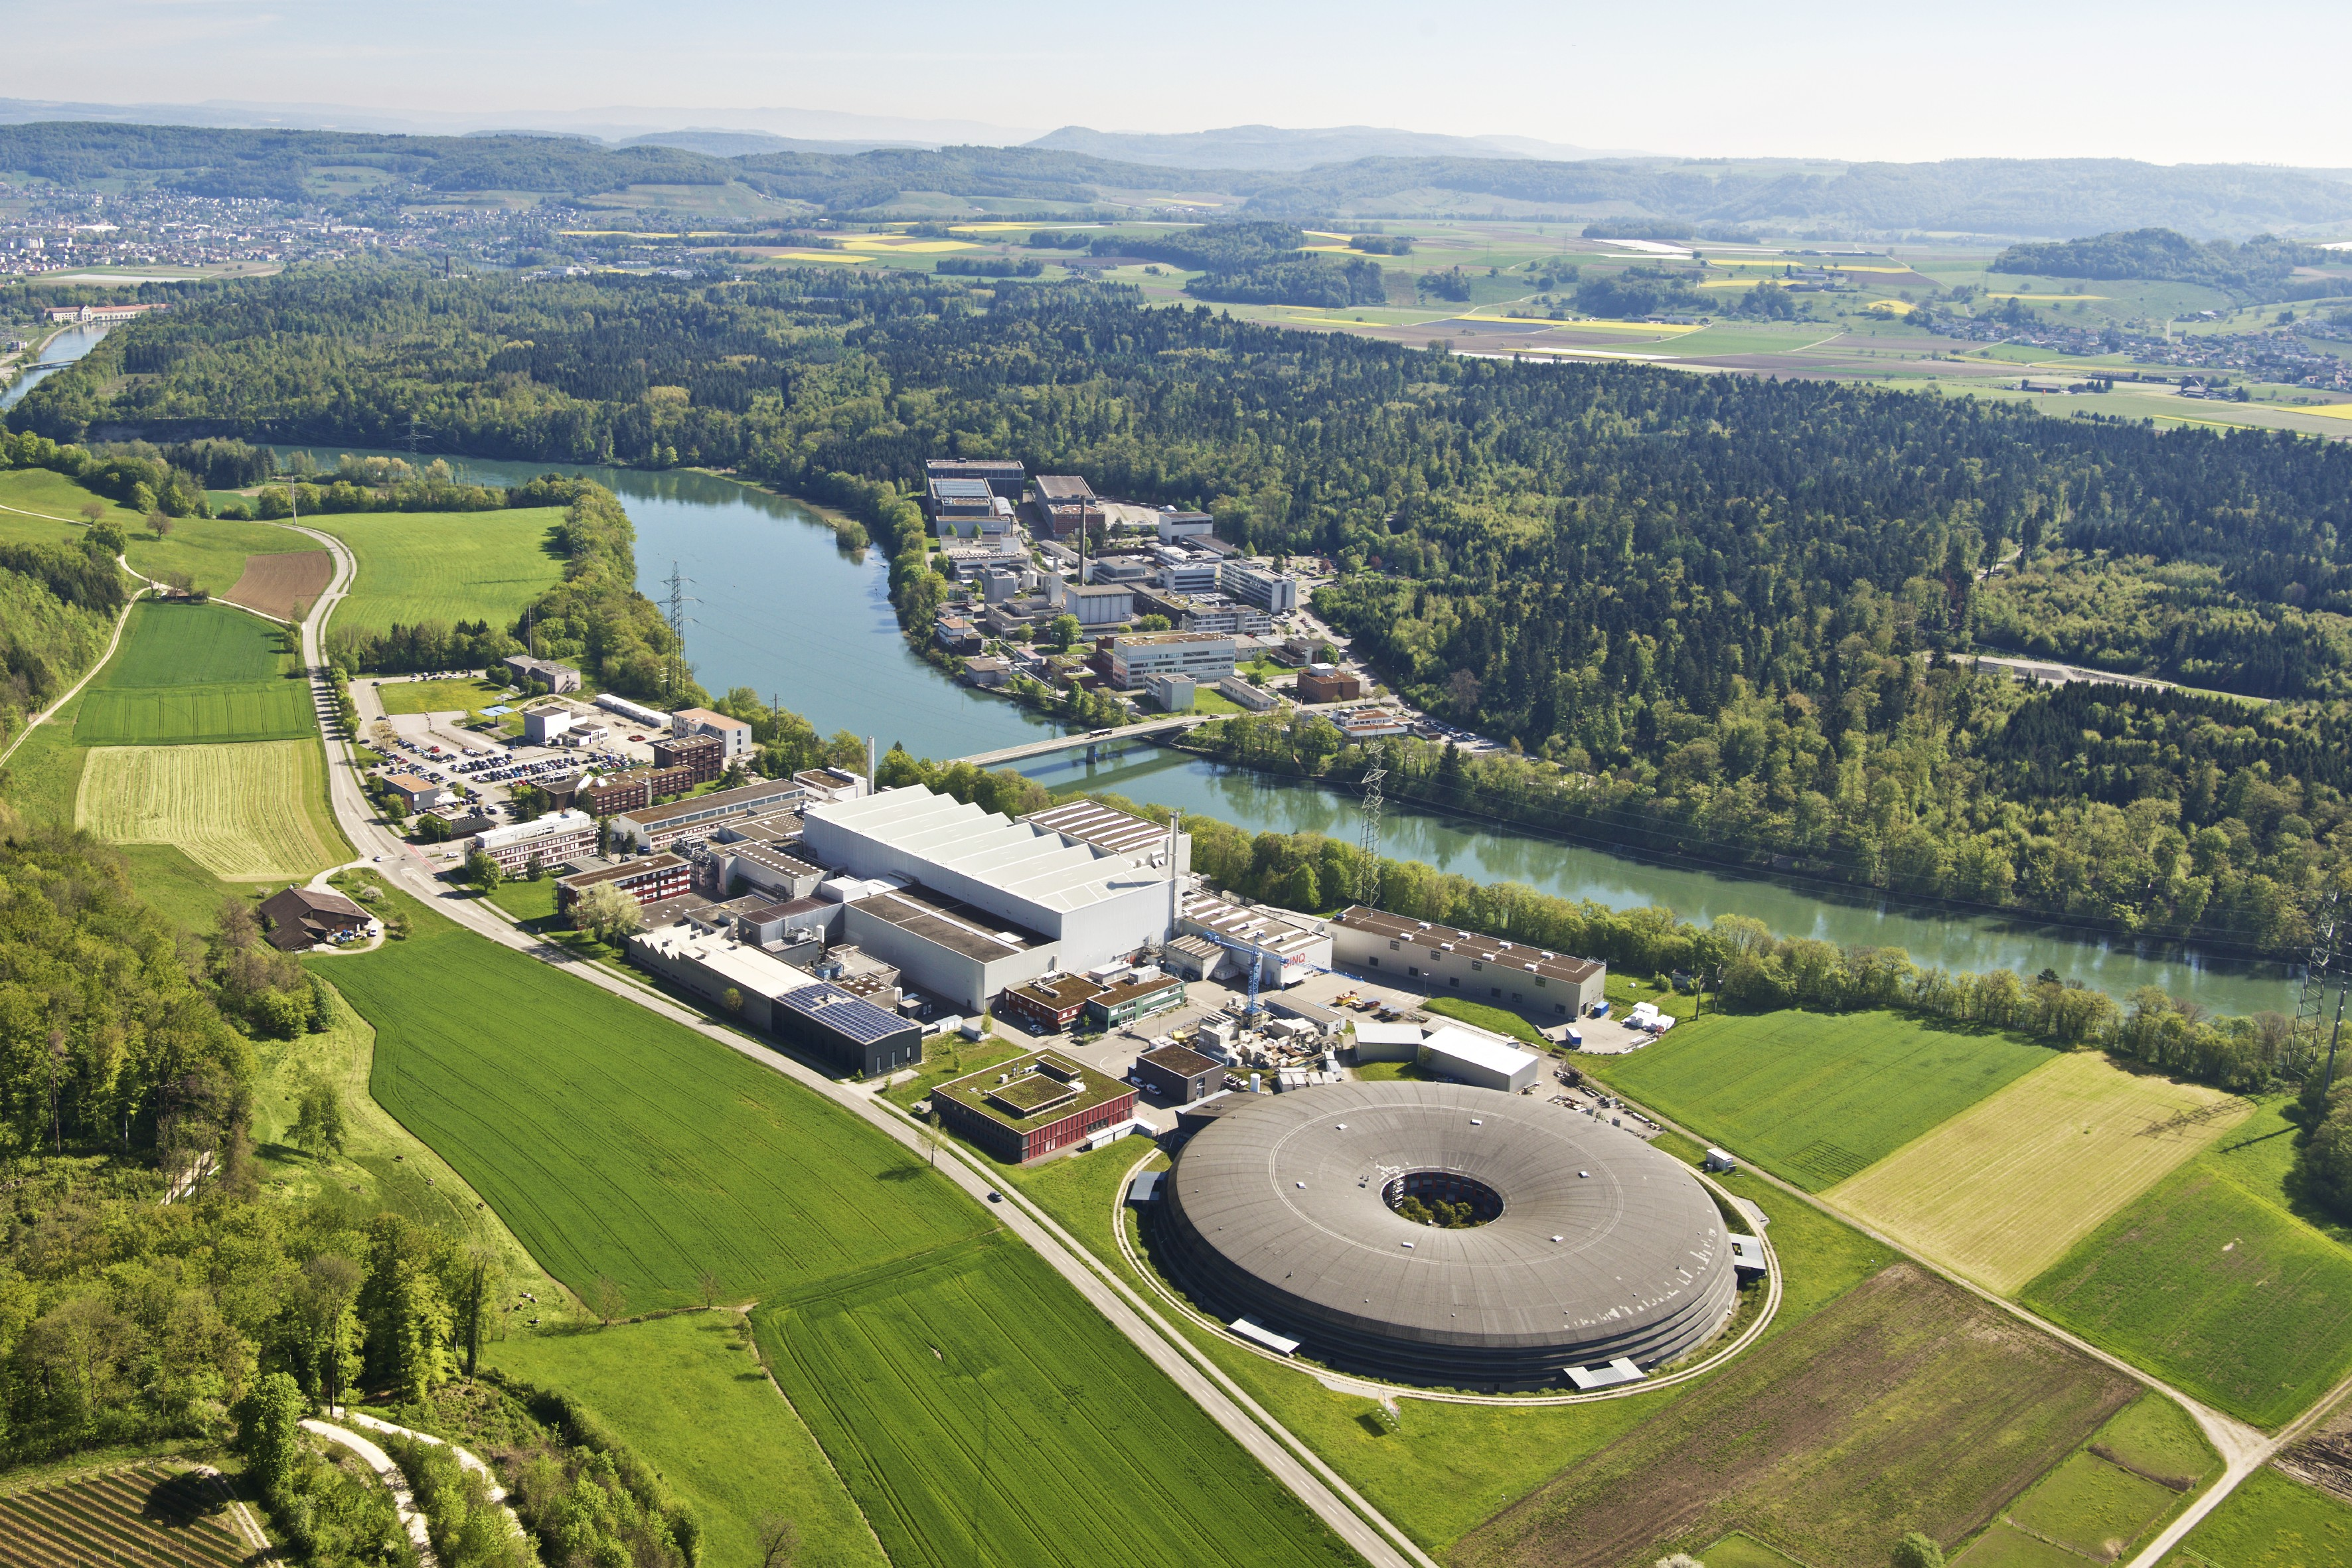
\includegraphics[width=\textwidth]{Chapitre1/figures/psi.jpg}
        \caption{A picture of the Paul Scherrer Institute. The SLS is the large circular building. 
         PSI has two main parts the East and West separated by the Aare river.}
        \label{fig:sls}
    \end{figure}

    \section{Detector's Group Presentation and Work}
    The Detector's Group is one of the research groups at the Paul Scherrer Institute. It is part of the Laboratory for X-ray Nanoscience and Technologies (LXN) which itself
    is part of the Center for Photon Science.

    % The group is composed of around 28 people, including the group leaders.
    The group is responsible for the development of new detectors, the maintenance of the existing ones, and the
    development of software for the data acquisition and analysis. 
    The group is also involved in the development of new techniques for the data analysis, such as image processing,
    pattern recognition, and machine learning.
    These Detector's are an integral part of the beamline's setup, and are used to detect the x-ray photons that are
    emitted by the synchrotron. Many experiments in different fields can use these detectors such as for studying the properties of materials \cite{butcher2024ptychographic},
    protein structures \cite{pomeranz2009crystal}, crystallography \cite{leonarski2023kilohertz}, biology \cite{lemcoff2023brilliant,dullin2024vivo}, and many other fields of research.

    On the software side, the group is responsible for the development of the software that is used to control the detectors, acquire the data, and analyze it.
    The software is developed in C++ and is used by scientists to perform their experiments.
    The main package maintained by the detector's group is the "SLS Detector Package" available publicly
    on \url{https://github.com/slsdetectorgroup/slsDetectorPackage}. The package provides several binaries such as:
    \begin{itemize}
        \item \textbf{slsReceiver} The receiver server acquires incoming data from detectors using UDP and listens for configurations from host machine using TCP.
        \item \textbf{slsDetectorGet} Used by the host machine to request the configuration on the Receiver or the Detector.
        \item \textbf{slsDetectorPut} Used to configure parameters on both the Receiver and Detector.
        \item \textbf{slsDetectorGui} A graphical user interface (GUI) that receives data from the Receiver and displays it.
    \end{itemize}
    The list of binaries is not exhaustive, and the package contains many other binaries for simulating detectors, analyzing data, and many other utilities.

    \begin{figure}[h]
        \centering
        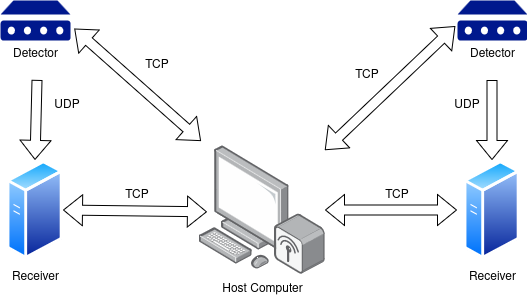
\includegraphics[scale=0.8]{Chapitre1/figures/slsreceiver.png}
        \caption{slsDetectorPackage setup for two detectors. Configuration uses TCP while
            data streaming from detector to slsReceiver uses UDP}
        \label{fig:detector}
    \end{figure}

    \section{Problem Statement}
    \subsection{Existing Solution}
    The detector's group includes scientists, software engineers, firmware engineers, chip designers and many more roles.
    The group is diverse and the libraries' usage differs from one user to another. In general the usage of the libraries includes: acquiring data from network
    , configuring receivers and detectors, storing incoming data, processing data on the fly or after storing it.
    For the standard functionalities users rely on the slsDetectorPackage binaries. But the slsDetectorPackage is a generic software
    developed for public use and has very broad functionalities. Hence, for specific use cases scientists might need to write their own scripts
    or change the slsDetectorPackage source code and build again.
    \subsection{Limits of The Existing Solution}
    The slsDetectorPackage is a very powerful software package, but it has some major limitations.
    \subsubsection{Code Complexity}
    First, the code is very complex and has a steep learning curve. The code is written in C++ and uses
    many advanced features of the language. The code is also very large, with around 200 thousand lines of code.
    This makes it difficult for new users to understand how the code works, and to modify it to suit their needs.
    In addition, scientists are not software engineers, and in case of a bug, new feature or a specific use case
    they will be exposed to complex code that they are not familiar with. This might include the need to understand
    C++ code, multi-threading, network programming, and many other advanced topics.


    \subsubsection{Code Rigidity}
    Second, the code is very rigid and inflexible. The code is designed to work in a specific way, and it is difficult
    to modify it to work in a different way. This means that scientists are limited in what they can do with the code,
    and they are forced to work within the constraints of the existing code. This can be very frustrating for scientists,
    who may have specific requirements that are not met by the existing code.
    Furthermore, some of the speicific use case implementations are very brittle and can break easily if the code is modified.
    It lacks proper testing, error handling and logging. This makes it difficult to maintain and extend the code.


    \subsubsection{Code Duplication}
    Third, the code is duplicated in many places. Scientist often rely on their own scripts to perform specific tasks.
    This leads to each scientist having their own version of the code, which is difficult to maintain and update.
    and also results in the use of sub-optimal code, which is not efficient or reliable.


    \subsubsection{Data Storage Limitations}
    As the detectors become more and more advanced, the amount of data that they produce is increasing.
    This has made processing the incoming data in real-time a must. The slsDetectorPackage provides limited
    functionalities for processing data on the fly. This means that scientists need to store the data on disk
    and process it later. This is not ideal and is becoming less practical as the amount of data can be very expensive to
    store and process. The new library should be designed to process around 10GB/s of data in real-time.

    \section{Project Goals}
    The goal of this project is to develop a new library that will address the limitations of the existing software.
    The new software package will be designed to be simple, flexible, and efficient. It will be easy to use, and will be
    designed to meet the needs of scientists and engineers. \\

    The library should include functionalities for acquiring data from receiver servers, stream data to receivers,
    read and write raw data files and numpy files, includes commonly used algorithms for data processing and it should
    expose a C++ and a Python API. \\

    In addition, code should be well tested, documented, and should include logging and error handling.
    The library should be designed to be extensible, so that new features can be added easily in the future.
    and also flexible so that it accomodates different and upcoming use cases. \\

    The library should be designed to be efficient, so that it can process data in real-time, and should be able to handle
    large amounts of data. It should use parallelism to distribute the load on multiple cores, and should be able to
    take advantage of the GPU for processing data. On the other hand it should abstract the low level details of the
    hardware and network communication to make it easy to use for the scientists.




    \section{Work Methodology}
    We used the \textbf{Kanban} methodology to manage the project. Kanban is a subsystem of the Toyota Production System (TPS),
    which was created in 1940s to control inventory levels, the production and
    supply of components, and in some cases, raw material. \cite{junior2010variations}

    The board is divided into several columns:
    \begin{itemize}
        \item \textbf{Backlog} Contains all the tasks that need to be done.
        \item \textbf{To Do} Contains the tasks that are ready to be worked on.
        \item \textbf{In Progress} Contains the tasks that are currently being worked on.
        \item \textbf{Done} Contains the tasks that are completed.
    \end{itemize}

    \subsection{Tools}
    We used Github Projects to manage the Kanban board. Github Projects is a tool that allows you to create a Kanban board
    and manage your tasks. It is integrated with Github, so you can link your tasks to your code, and track your progress
    easily. We also used Github Issues to create tasks, and Github Pull Requests to review and merge the code.

    The Kanban boards were available for all the group members (involved in project or not), so that they can see the progress
    of the project, and contribute to it if needed. The boards were updated regularly, and the progress was tracked using the
    boards. The boards were also used to plan the work, and to assign tasks to the group members.

    \subsection{Benefits of Kanban}
    The Kanban methodology has several benefits:
    \begin{itemize}
        \item \textbf{Visibility} The Kanban board provides a visual representation of the work
              that needs to be done, and the progress that has been made.
        \item \textbf{Flexibility} The Kanban board is flexible, and can be easily adapted to
              the needs of the project.
        \item \textbf{Efficiency} The Kanban board helps to prioritize the work, and to focus
              on the most important tasks.
        \item \textbf{Collaboration} The Kanban board is a collaborative tool, and can
              be used by all the group members to track the progress of the project.

    \end{itemize}

    \subsection{Meetings}
    We had regular meetings with the group members to discuss the progress of the project, and to plan the work.
    On each Tuesday, The whole group meets for about an hour to discuss the progress of the multiple projects that are being worked on.
    This meeting helps to keep everyone informed about the progress of the projects, and to identify any issues that need to be addressed.

    In addition, on each Friday, a one-on-one meeting is held with the project supervisor to discuss the progress made during the week,
    and to plan the work for the next week. This is a more detailed meeting where we discuss the tasks that need to be done, and the
    kep track of the progress of the project.

    Furthermore, the group has an open door policy, where anyone can ask for help, or discuss any issues that they are facing.
    Knowledge sharing is encouraged, and regular short discussions help overcoming the roadblocks that one might encounter.
    \section{High Level Planning}
    Even though the work methodology is highly flexible, we have a high level planning that we follow.
    The project is divided into several phases:
    \begin{itemize}
        \item \textbf{Phase 1: Research and Project Setup} In this phase, we researched the existing solutions, identified the limitations of the existing software,
              setup the project, and developed a high level architecture for the new library.
        \item \textbf{Phase 2: Implementation of the File Module} In this phase, we implemented the file IO module, which is responsible for reading and writing raw data files and numpy files.
        \item \textbf{Phase 3: Implementation of the Network Module} In this phase, we implemented the network module, which is responsible for acquiring data from receiver servers, and streaming data.
        \item \textbf{Phase 4: Implementation of the Processing Module} In this phase, we implemented the processing module, which includes commonly used algorithms for data processing.
        \item \textbf{Phase 5: Implementation of the Python API} In this phase, we implemented the Python API, which allows users to use the library from Python.
        \item \textbf{Phase 6: Documentation, Testing and Evaluation} In this phase, we tested the library more thoroughly, evaluated the performance, documented the code and added tutorials.
    \end{itemize}

    It is important to note that the phases are not fixed, and can be adapted to the needs of the project. The phases are used to plan the work, and to track the progress of the project.
    For example the python API was implemented in parallel with the other modules, as it was very useful to test the library and to get feedback from the users.

    \begin{figure}[h]\centering
        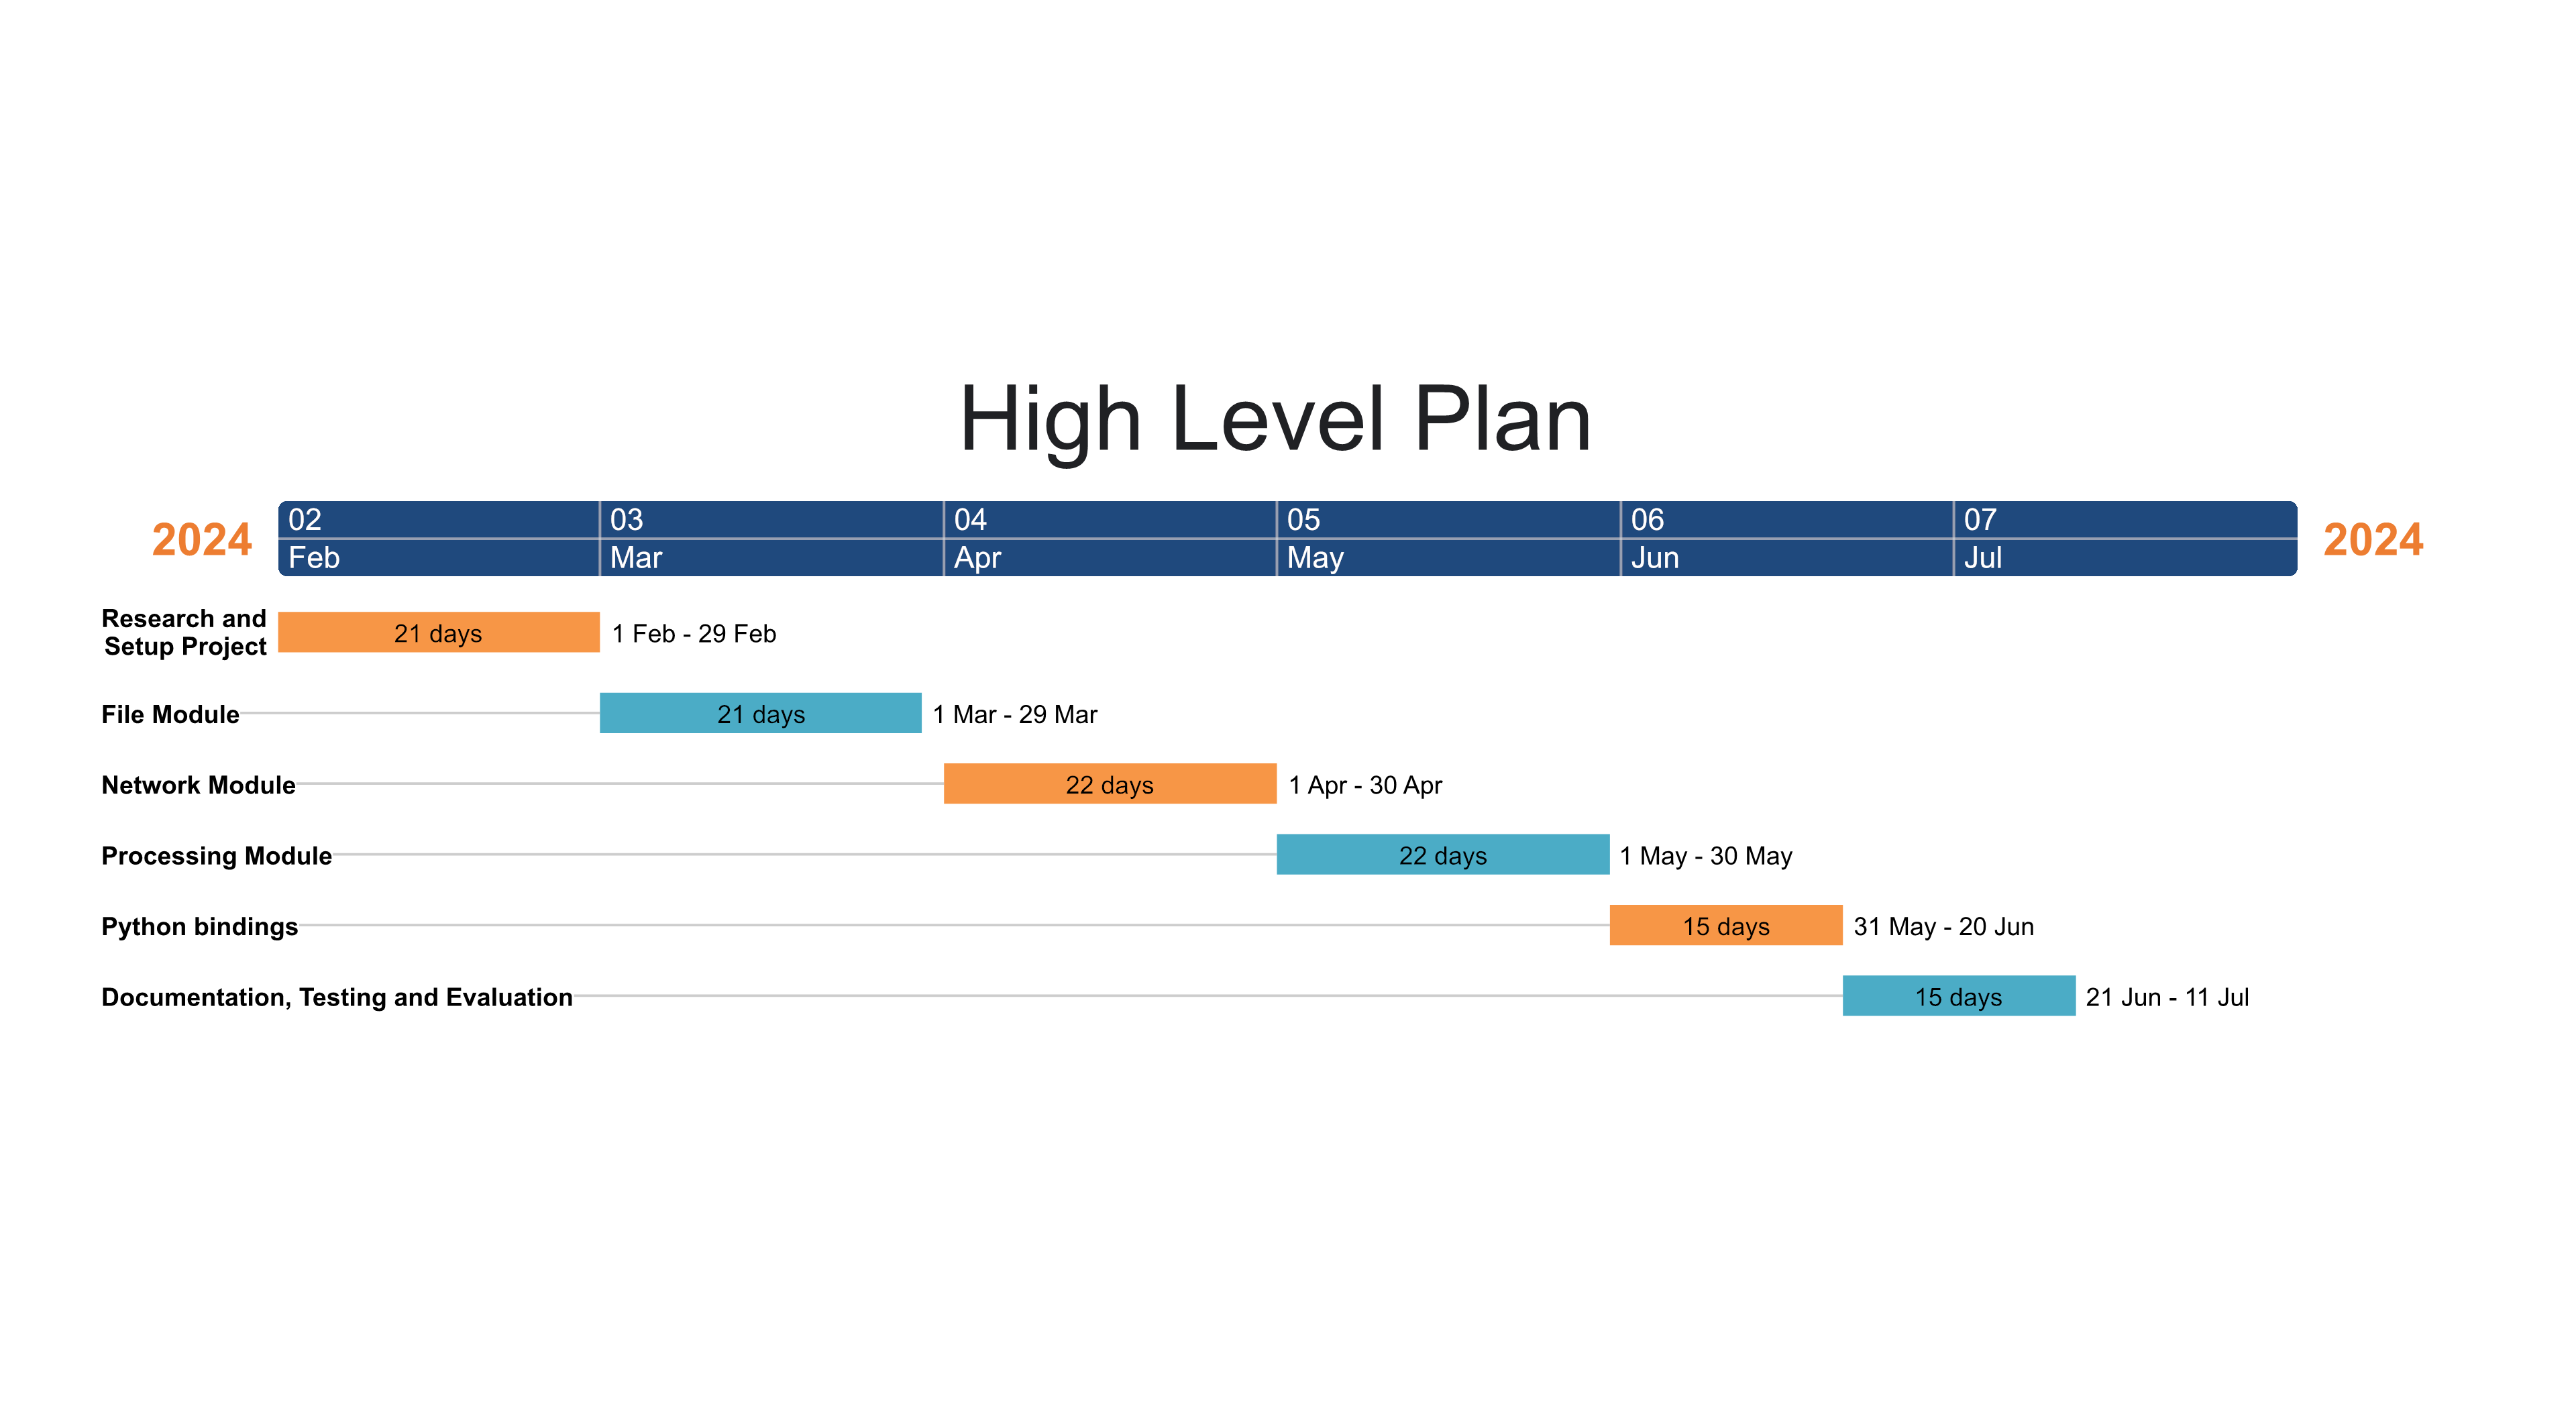
\includegraphics[width=\textwidth]{Chapitre1/figures/gantt.png}
        \caption{Gantt Diagram of the 6 phases of development. A margin was left at the end of the project to account for 
        holidays, vacation days and development delays}
        \label{fig:gantt}
    \end{figure}

    \section*{Conclusion}
    In this chapter we presented the host company and the key difficulties faced 
    by its detectors group. Following this we established the goals of the project
    and the methodology that we will follow to achieve them. 


    %==============================================================================
\end{spacing}

\part{Partie 2}

\setcounter{chapter}{1}
\chapter{Design}
\graphicspath{{Chapitre2/figures/}}

%\DoPToC

%==============================================================================
\pagestyle{fancy}
\fancyhf{}
\fancyhead[R]{\bfseries\rightmark}
\fancyfoot[R]{\thepage}
\renewcommand{\headrulewidth}{0.5pt}
\renewcommand{\footrulewidth}{0pt}
\renewcommand{\chaptermark}[1]{\markboth{\MakeUppercase{\chaptername~\thechapter. #1 }}{}}
\renewcommand{\sectionmark}[1]{\markright{\thechapter.\thesection~ #1}}

\begin{spacing}{1.2}
%==============================================================================
\section*{Introduction}
La partie conception de l'application \textbf{\textsl{n'est pas toujours obligatoire}}. En effet, quand notre travail consiste en une étude théorique, ou une mise en place d'un système par exemple, 
il est inutile voire obsolète de faire un diagramme de classes ou de séquence.\\
Quand il s'agit de développement, par contre, la partie conception s'impose. 
\section{Recommadations}
En général, 
il faut suivre les règles suivantes :
\begin{itemize}
	\item Choisir une méthodologie de travail : un processus unifié, une méthode agile;
\end{itemize}
\section{Diagrammes}
Il faut Bien choisir les diagrammes adéquats pour votre application. En général, les
diagrammes obligatoires sont les diagrammes de cas d'utilisation, de classe et de 
séquence. Vous pouvez ajouter en plus le diagramme qui vous semble pertinent :
par exemple, pour une application sur plusieurs tiers, il est intéressant de
montrer le diagramme de déploiement;
\begin{itemize}

\item Les diagrammes doivent être clairs, lisibles et bien expliqués, sans pour autant
nous submerger de détails. Des explications trop longues deviennent ennuyeuses;
\item Si un diagramme est trop grand, vous pouvez le diviser, le représenter sous
forme de plusieurs diagrammes, ou vous abstraire de certains détails. Si c'est
impossible, imprimez le sur une grande page (A3), quitte à la plier ensuite. Le
plus important est que tous les mots soient lisibles.

\end{itemize}
\subsection{Diagramme de Séquence}
Un diagramme de séquence :
\begin{itemize}
	\item Représente un scénario possible qui se déroule dans un cas d'utilisation. 
	Vous n'êtes donc pas obligés de montrer tous les cas d'exécution possibles;
	\item Représente l'interaction entre les objets : donc normalement, toutes les
	instances définies dans un diagramme de séquences doivent correspondre 
	 à des classes qui se trouvent dans le diagramme des classes;
	 \item Il existe parfois des dizaines de diagrammes de séquences possibles. Choisissez certains d'entre eux à mettre dans le rapport (2 ou 3). Privilégiez les diagrammes les plus importants (et non, l'authentification n'en fait pas partie!).
\end{itemize}
\subsection{Diagramme de Classes}
Un diagramme de classes :
\begin{itemize}
\item Doit être fidèle à l'architecture logicielle choisie. Si vous utilisez le MVC, 
alors les trois couches doivent être représentées dans le diagramme de classes grâce aux packages;
\item Les stéréotypes sont fortement conseillés. Si vous développez une
application web, n'hésitez pas à utiliser les stéréotypes de la figure \ref{fig:fig2} : 
\begin{figure}[!ht]\centering

\includegraphics[scale=0.9]{stereotypes.jpg}
\caption{Les stéréotypes}
\label{fig:fig2}
\end{figure}
\item Attention à ne pas confondre classes et tables : évitez la tentation de
mettre des id partout.

\end{itemize}
 
\section*{Conclusion}
Faire ici une petite récapitulation du chapitre, ainsi qu'une introduction du chapitre suivant.





%==============================================================================
\end{spacing}


\setcounter{chapter}{2}
\chapter{Implementation of a Flexible Data Analysis Library for Hybrid X-ray Particle Detectors }
\minitoc %insert la minitoc
\graphicspath{{Chapitre3/figures/}}

%\DoPToC
%==============================================================================
\pagestyle{fancy}
\fancyhf{}
\fancyhead[R]{\bfseries\rightmark}
\fancyfoot[R]{\thepage}
\renewcommand{\headrulewidth}{0.5pt}
\renewcommand{\footrulewidth}{0pt}
\renewcommand{\chaptermark}[1]{\markboth{{\chaptername~\thechapter. #1 }}{}}
\renewcommand{\sectionmark}[1]{\markright{\thechapter.\thesection~ #1}}

\begin{spacing}{1.2}

    %==============================================================================
    \section*{Introduction}
    In this chapter we will go through the implementation and design choices for each module.

    \section{Project Setup}
    \subsection{Project Structure}
    \begin{figure}[hb]
        \centering
        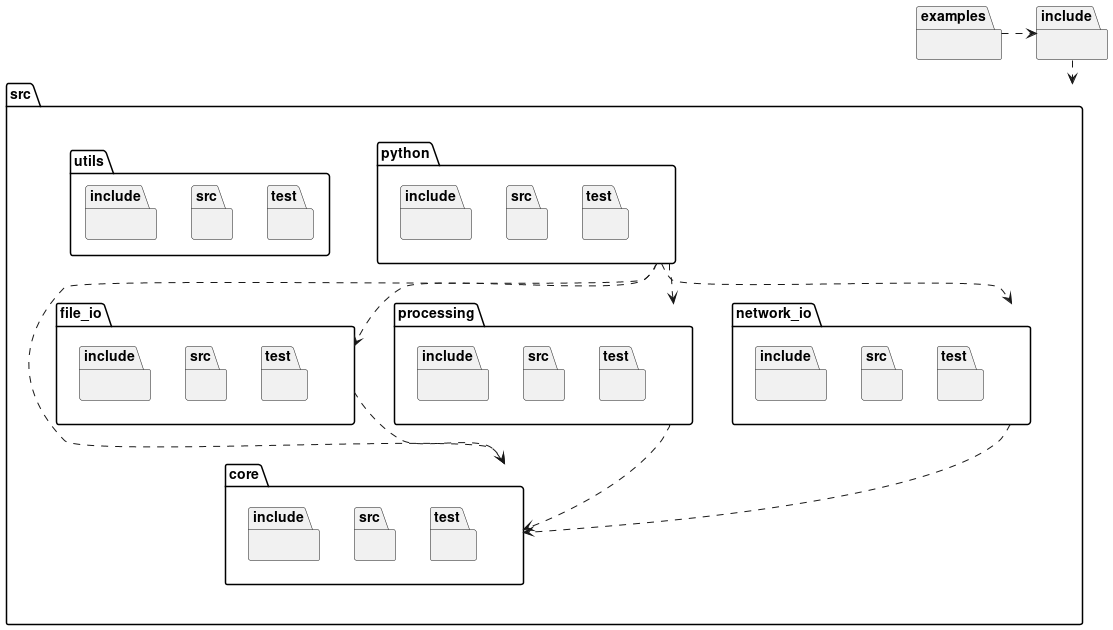
\includegraphics[width=0.8\textwidth]{Chapitre3/figures/folders.png}
        \caption{Project folder structure}
        \label{fig:folders}
    \end{figure}
    The folder structure of the project is shown in Figure \ref{fig:folders}. The file hierarchy
    is based on the Pitchfork project structure recommendations \cite{pitchfork}.
    The project is composed of a include folder containing the header files,
    a src folder containing the source files,
    an examples folder containing the examples.
    The root directory of the project contains a CMakeLists.txt file which is used to build the project.
    Each module has its own folder in the src directory.
    For example the core module has include, src and test folders inside it.




    \subsection{Build System}
    The project uses CMake as the build system. CMake is a cross-platform build system that
    generates native build files for the platform of your choice. It is a powerful tool that
    can be used to build, test and package software. The CMakeLists.txt file in the root directory
    of the project is used to configure the project. Each module also has its own CMakeLists.txt
    file which is used to configure the module and build the sources files and tests. CMake will compile
    each module independently as static libraries and link them together to create the final
    executables or share objects.\\

    In this project CMake is also used to manage the dependencies. The project uses external
    libraries such as ZeroMQ, FMT, Catch2... CMake downloads and builds these libraries
    automatically. This is done using the FetchContent module in CMake. The FetchContent module
    allows to download and build external projects at configure time.

    \subsection{Version Control}
    The project uses Git as the version control system. Git is a distributed version control system
    that allows tracking changes in the source code. It is a powerful tool that allows multiple people
    to work on the same project at the same time.\\

    The remote repository is hosted on GitHub. GitHub is a web-based platform that provides
    hosting for software development version control using Git. It also provides collaboration
    features such as bug tracking, feature requests, task management and wikis for every project.
    Pull requests are used to merge changes from one branch to another. This allows reviewers
    to check the code before it is merged into the main branch.\\



    \subsection{Testing and Continuous Integration}
    The project uses Catch2 as the testing framework. Catch2 is a modern, C++-native, header-only,
    test framework for unit-tests. It is easy to use and provides a lot of features such as
    BDD-style testing, test cases, sections, assertions, tags, test fixtures, test cases
    and test suites.\\

    Each module has its own test folder containing the test files. The test files are compiled
    into a test executable which is run to test the module. The test executable is built using
    the CMakeLists.txt file in the test folder of the module. A single test executable is built
    for the whole library which runs all the tests of the submodules. Tags can be used to run or exclude
    specific groups of tests.\\

    Continuous integration is used to automatically build and test the project. GitHub Actions
    is used to run the tests on each push to the repository. The tests are run on multiple
    platforms including Windows, Linux and MacOS. And different configurations are used such
    as Debug and Release, with and without Python bindings, download dependencies with CMake or use system libraries...
    Furthermore, the code is checked for formatting using clang-format and for linting checks using clang-tidy.
    Linting checks are used to find potential bugs and code smells in the code.\\



    \subfile{Chapitre3/part1.tex}

    \section{Processing Module Implementation}
    \begin{figure}
        \centering
        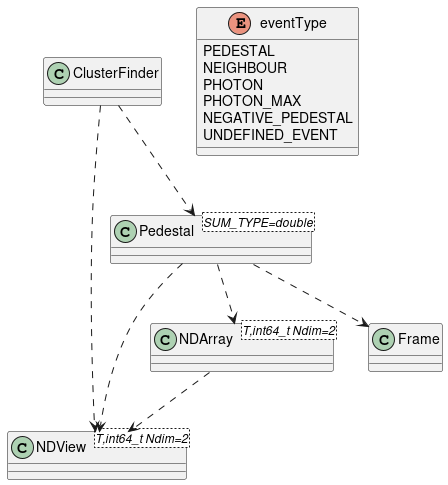
\includegraphics[width=0.8\textwidth]{Chapitre3/figures/processing_class.png}
        \caption{Processing module}
        \label{fig:processing}
    \end{figure}

    The processing module contains the classes and algorithms used to process the data.
    The class diagram of the processing module is shown in Figure \ref{fig:processing}.
    Currently two data processing algorithms are implemented.

    \subsection{Pedestal class}

    The pedestal algorithm is used for preprocessing the incoming frame data. Detectors have a
    background signal that is present even when no particles are detected. This background signal
    can be the still image of the sample. The Pedestal substraction algorithm is used to remove
    this background signal and help in the detection of key meaningful signals. The Pedestal class
    is used to calculate the pedestal values for each pixel. Usually the pedestal values are
    calculated by taking the average of the last N frames. However, in our case we a frame of data
    can have 1024x1024 pixels keeping track of the last N frames would be memory intensive i.e
    $O(N)$ in memory.
    In order to store the last 1000 frames for the average $1024*1024*1000*4 = 4GB$  of memory would be needed.
    Instead we keep track of the sum of the last N frames and with each new frame we subtract the
    average of the last N frames and add the new frame.
    \begin{equation}
        \text{Sum}_i = \text{Sum}_{i-1} - \frac{\text{Sum}_{i-1}}{N} + \text{Frame}_i
    \end{equation}
    \begin{equation}
        \text{Pedestal}_i = \frac{\text{Sum}_i}{N}
    \end{equation}

    This way we only need to store the sum of the last N frames
    which is $1024*1024*4 = 4MB$ of memory.  In addition this method is faster, more stable
    and $O(1)$ in terms of memory and time complexity.


    \subsection{ClusterFinder class}
    After substracting the pedestal values from the incoming frame data, the next step is to
    find the clusters of pixels that are hit by the incoming particles. For photon particles
    a fixed size cluster of 2x2 or 3x3 is used as a sliding window to find the appropriate   particle hits.
    For electrons, as they usually leave a trail behind, a flood fill algorithm is used to find the
    clusters of adjacent pixels that are hit by the incoming particles.\\


    \section{Python Bindings Implementation}
    Writing python code is a lot of fun and very productive. It is a high-level language that is
    easy to learn and use. It is also very popular in the scientific community. It is used for
    data analysis, machine learning, artificial intelligence, web development, automation and many more.

    However, Python is an interpreted language and it is very dynamic. this makes it slower than
    compiled languages like C++. \\

    On the other hand, C++ is a compiled language that is very fast and efficient. It is used to
    write high-performance code that is used in games, operating systems, databases, web servers
    , financial systems and many more.

    It is also very complicated and hard to learn and use. It is strongly typed and has a lot of
    boilerplate code.\\

    Ideally, we would like to write the core of our library in C++ and then use it in Python.
    This is where Python bindings come in. Python bindings are used to expose C++ code to Python.
    There are many ways to create Python bindings such as SWIG, Boost.Python, pybind11, ctypes, CFFI...

    In this project, we use pybind11 to create the Python bindings. pybind11 is a lightweight header-only
    library that exposes C++ code to Python.
    It is influenced by the Boost.Python library, But it presents itself as bloat free alternative.
    It is easy to use and provides a lot of features such as
    automatic type conversion, exception handling, class inheritance, function overloading, lambda functions and
    integrates NumPy support.

    pybind11 is heavily used in numerical/ML libraries such as scipy, Tensorflow, JAX, Pytorch\dots\\

    The pybind11 creates an extension module that can be imported in Python. The extension module
    contains the C++ code that is exposed to Python. After compiling and linking pybind11 produces
    a dynamic library (dynamic load) that can be used by Python. The dynamic library is loaded
    at runtime and the C++ code is executed in the Python interpreter.\\

    \begin{lstlisting}[language=C++, caption=Example of a C++ binding for the Frame class,label=lst:frame_binding]
py::class_<Frame>(m, "Frame", py::buffer_protocol())
    .def(py::init<std::byte *, int64_t, int64_t, Dtype>())
    .def(py::init<int64_t, int64_t, Dtype>())
    .def_property_readonly("rows", &Frame::rows)
    .def_property_readonly("cols", &Frame::cols)
    .def_property_readonly("bitdepth", &Frame::bitdepth)
    .def_property_readonly("size", &Frame::bytes)
    .def_property_readonly("data", &Frame::data, py::return_value_policy::reference)
    .def_buffer([](Frame &f) -> py::buffer_info {
        Dtype dt = f.dtype();
        return {
            f.data(),                           /* Pointer to buffer */
            static_cast<int64_t>(dt.bytes()),   /* Size of one scalar */
            dt.format_descr(),                  /* Python struct-style format descriptor */
            2,                                  /* Number of dimensions */
            {f.rows(), f.cols()},               /* Buffer dimensions */
            {f.cols() * dt.bytes(), dt.bytes()} /* Strides (in bytes) for each index */
        };
});

        
    \end{lstlisting}

    Listing \ref{lst:frame_binding} shows an example of a C++ binding for the Frame class.
    \lstinline|.def()| method is used to define a class method. In the example, we defined 
    the constructor with it. \lstinline|.def_property_readonly()| is used to define a read-only property.
    \lstinline|.def_buffer()| is used to define a buffer protocol. The buffer protocol is used to expose
    the data of the Frame class to Python. This protocol is very useful when working with NumPy arrays 
    as it allows us to convert a Frame object to a NumPy array with or without copying the data.\\

    \begin{lstlisting}[language=Python, caption=Example of using the Frame class in Python,label=lst:frame_python]
import numpy as np # import numpy
import aare        # import the aare library

frame = aare.Frame(1024, 1024, aare.Dtype.UINT16) # create a frame object
rows = frame.rows # get the number of rows
array = np.array(frame.data, copy=False) # convert the frame object to a numpy array
    \end{lstlisting}

    Listing \ref{lst:frame_python} shows an example of using the Frame class in Python.
    As we can see the Frame class is used as a normal Python class. Furthermore, we can 
    manipulate the data of the Frame object as a NumPy array. This is very useful as it allows
    us to use the Frame object with other libraries that use NumPy arrays.\\


    \section*{Conclusion}
    In this chapter, we went through the implementation of the project. We discussed the 
    project setup and we dived deep into the details of the implementation. We dived into
    the design choices that were made in order to juggle between performance, flexibility, 
    and usability. 

    %==============================================================================
\end{spacing}


\backmatter
\pagestyle{fancy}
\fancyhf{}
\renewcommand{\chaptermark}[1]{\markboth{Conclusion and Perspectives}{}}
\fancyhead[R]{Conclusion and Perspectives}
\fancyfoot[R]{\thepage}
\renewcommand{\headrulewidth}{0.5pt}
\renewcommand{\footrulewidth}{0pt}
\chapter{Conclusion and Perspectives}
%==============================================================================
\pagestyle{fancy}
\fancyhf{}
\fancyhead[R]{\bfseries\rightmark}
\fancyfoot[R]{\thepage}
\renewcommand{\headrulewidth}{0.5pt}
\renewcommand{\footrulewidth}{0pt}
\renewcommand{\chaptermark}[1]{\markboth{\MakeUppercase{\chaptername~\thechapter. #1 }}{}}
\renewcommand{\sectionmark}[1]{\markright{\thechapter.\thesection~ #1}}

\begin{spacing}{1.2}
%==============================================================================

C'est l'une des parties les plus importantes et pourtant les plus négligées 
du rapport. Ce qu'on \underline{ne veut pas voir} ici, c'est combien ce stage vous a été bénéfique, comment il vous a appris à vous intégrer, à connaître le monde du travail, etc.\\
Franchement, personne n'en a rien à faire, du moins dans cette partie. Pour cela, vous 
avez les remerciements et les dédicaces, vous pourrez vous y exprimer à souhait.\\
La conclusion, c'est très simple : c'est d'abord le résumé de ce que vous avez raconté
dans le rapport : vous reprenez votre contribution, en y ajoutant ici les outils que vous 
avez utilisé, votre manière de procéder. Vous pouvez même mettre les difficultés
rencontrées. En deuxième lieu, on y met les perspectives du travail : ce qu'on pourrait 
ajouter à votre application, comment on pourrait l'améliorer.

%==============================================================================
\end{spacing}

\singlespacing
% \renewcommand{\bibname}{References}
\printbibliography

\onehalfspacing

\appendix
\setcounter{figure}{0} 
\setcounter{table}{0}
\setcounter{footnote}{0}
\setcounter{equation}{0}
\pagestyle{fancy}
\fancyhf{}
\renewcommand{\chaptermark}[1]{\markboth{\MakeUppercase{#1 }}{}}
\renewcommand{\sectionmark}[1]{\markright{\thesection~ #1}}
\fancyhead[RO]{\bfseries\rightmark}
\fancyhead[L]{\bfseries\leftmark}
\fancyfoot[RO]{\thepage}
\fancyfoot[L]{\thepage}
\renewcommand{\headrulewidth}{0.5pt}
\renewcommand{\footrulewidth}{0pt}

\makeatletter
\renewcommand\thefigure{A.\arabic{figure}}
\renewcommand\thetable{A.\arabic{table}} 
\makeatother

\chapter{Appendix : Miscellaneous remarks}
\graphicspath{{Annexe1/figures/}}
%==========================================================================

%    Annexe

%===========================================================================
\begin{itemize}
\item Un rapport doit toujours être bien numéroté;
\item De préférence, ne pas utiliser plus que deux couleurs, ni un caractère fantaisiste; 
\item Essayer de toujours garder votre rapport sobre et professionnel; 
\item Ne jamais utiliser de je ni de on, mais toujours le nous (même si tu as tout fait tout seul); 
\item Si on n'a pas de paragraphe 1.2, ne pas mettre de 1.1;
\item TOUJOURS, TOUJOURS faire relire votre rapport à quelqu'un d'autre (de préférence qui n'est pas du domaine) pour vous corriger les fautes d'orthographe et de français;
\item Toujours valoriser votre travail : votre contribution doit être bien claire et mise en évidence; 
\item Dans chaque chapitre, on doit trouver une introduction et une conclusion;
\item Ayez toujours un fil conducteur dans votre rapport. Il faut que le lecteur suive un raisonnement bien clair, et trouve la relation entre les différentes parties;
\item Il faut toujours que les abréviations soient définies au moins la première fois où elles sont utilisées. Si vous en avez beaucoup, utilisez un glossaire.
\item Vous avez tendance, en décrivant  l'environnement matériel, à parler de votre ordinateur, sur lequel vous avez développé : ceci est inutile. Dans cette partie, on ne cite que le matériel qui a une influence sur votre application. Que vous l'ayez développé sur Windows Vista ou sur Ubuntu n'a aucune importance;
\item Ne jamais mettre de titres en fin de page; 
\item Essayer toujours d'utiliser des termes français, et éviter l'anglicisme. Si certains termes  sont plus connus en  anglais, donner leur équivalent en français la première fois que vous les utilisez, puis utilisez le mot anglais, mais en italique;
\item Éviter les phrases trop longues : clair et concis, c'est la règle générale !\\

\newpage

\textbf{Rappelez vous que votre rapport est le visage de votre travail : un mauvais rapport peut éclipser de l'excellent travail. Alors prêtez-y l'attention nécessaire.}

 
\begin{figure}[!ht]\centering

\includegraphics[scale=0.5]{ingenieur.jpg}
\end{figure}
\end{itemize}




\end{document}